\smalltitle{سوال 5}
\begin{center}
    \textbf{
    با توجه به اینکه تمامی ورودی‌ها بجز تعداد ورودی محدود باز هستند، پس تنها راه منع خدمت ورود از آن مسیرها است پس 
    برای جلوگیری از dos در هر قسمت موقع تعریف قوانین آن روش جلوگیری از 
    داس زدن روی آن مورد را نیز بیان می‌کنیم}
\end{center}
برای حل این سوال ابتدا باید ترافیک ورودی را کامل ببندیم.
\begin{latin}
\begin{lstlisting}
sudo iptables -P INPUT DROP
\end{lstlisting}
\end{latin}
\begin{center}
    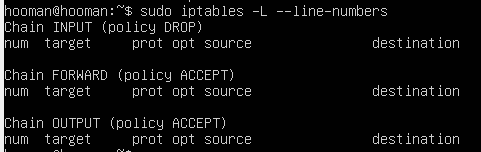
\includegraphics[scale=0.45]{pics/iptables1.png}
\end{center}
سپس باید ورودی‌های کانکشن‌های Establish شده را باز کنیم.
\begin{latin}   
\begin{lstlisting}
sudo iptables -A INPUT -m conntrack --ctstate ESTABLISHED -j ACCEPT
\end{lstlisting}
\end{latin}
می‌توانیم تست کنیم که آیا قانون ما درست کار می‌کند یا خیر.
برای این کار از nc استفاده می‌کنیم تا ببینیم در صورت 
وصل شدن به بیرون آیا می‌توانیم کانکشن ایجاد کنیم یا خیر.همانطور که از عکس مشاهده می‌کید توانسته‌ایم از ای پی مورد نظر به ای پی دیگر با استفاده از nc وصل 
شویم و یک پیام نیز بفرستیم.
\begin{center}
    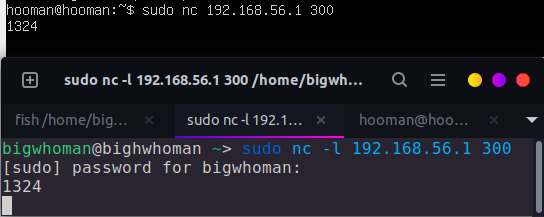
\includegraphics[scale=0.40]{pics/iptables2.png}
\end{center}
سپس باید قوانین ضد dos را تنظیم کنیم تا اگر 
فردی با کانکشن‌های ورودی سعی به dos کردن ما داشت جلوی وی گرفته شود.
دستورات زیر را استفاده می‌کنیم.
\begin{latin}   
\begin{lstlisting}
sudo iptables -A INPUT -p tcp -m connlimit --connlimit-above 3 --connlimit-mask 32 -j REJECT
\end{lstlisting}
\end{latin}
با این کار عملا اجازه داده نمی‌شود یک ای پی بیش از ۳ 
درخواست در دقیقه برای ما ارسال کند.
حال باید پورت ssh یا همان پورت ۲۲ را باز کنیم اما 
برای این کار باید ابتدا مطمئن شویم کسی به این پورت عملا حمله نمی‌کند و پورت را بروت فورس نمی‌کند. 
برای این کار دستورات زیر را می‌زنیم : 
\begin{latin}   
\begin{lstlisting}
sudo iptables -A INPUT -p tcp --dport 22 -m conntrack --ctstate NEW -m recent --set
sudo iptables -A INPUT -p tcp --dport 22 -m conntrack --ctstate NEW -m recent --update --seconds 60 --hitcount 10 -j DROP
sudo iptables -A INPUT -p tcp --dport 22 -m conntrack --ctstate NEW,ESTABLISHED -j ACCEPT
\end{lstlisting}
\end{latin}
در ۳ دستور بالا، اولین دستور عملا کانکشن‌هایی که به پورت ۲۲ زده می‌شوند را ضبط می‌کند، دومی می‌گوید در هر ۶۰ ثانیه فقط ۱۰ کانکشن جدید به این پورت می‌تواند زده شود و سومی عملا می‌گوید پورت ۲۲ آماده کانکشن زدن است.
اگر فردی با یک ای پی سعی کند در دقیقه بیش از 
۱۰ کانکشن با پورت ۲۲ برقرار کند، عملا کانکشن وی 
دراپ می‌شود. در عکس زیر می‌توانید این را ببینید.
\begin{center}
    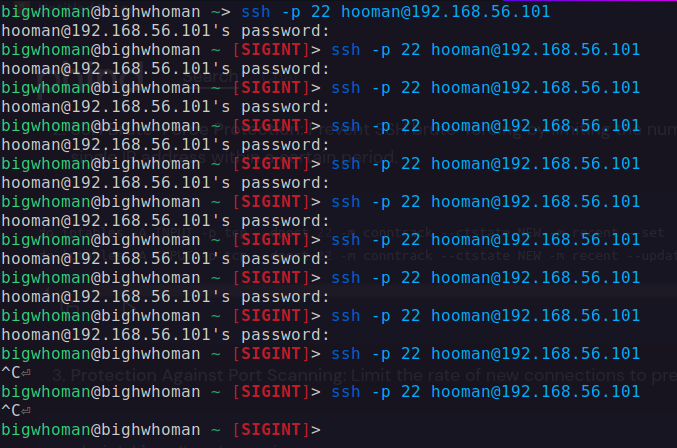
\includegraphics[scale=0.30]{pics/iptables3.png}
\end{center}
در قسمت بعدی باید طوری تنظیم کنیم که پکت‌های icmp اجازه ورود داشته باشند اما حمله 
\lr{icmp flood} نیز 
رخ ندهد و همچنین اجازه \lr{icmp redirect} را ندهیم.
برای این کار کامندهای زیر را استفاده می‌کنیم.
\begin{latin}   
\begin{lstlisting}
sudo iptables -A INPUT -p icmp --icmp-type redirect -j DROP
sudo iptables -A INPUT -p icmp --icmp-type echo-request -m limit --limit 1/second --limit-burst 1 -j ACCEPT
sudo iptables -A INPUT -p icmp --icmp-type echo-request -j DROP
\end{lstlisting}
\end{latin}
اولین قانون بالا می‌گوید icmp ها از مدل redirect را کلا دراپ کن 
در قسمت بعدی نیز می‌گوییم که کلا ۱ درخواست icmp در ثانیه می‌تواند به سیستم وارد شود و در غیر این صورت 
خط بعدی اجرا شده و درخواست icmp رد می‌شود. 
عکس زیر نشان می‌دهد که در قسمت اول جواب بسته icmp امده و در قسمت 
بعدی پکت icmp دراپ شده است چون فاصله بین دو درخواست کمتر از ۱ ثانیه است.
\begin{center}
    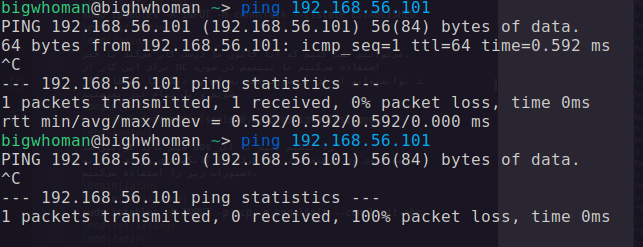
\includegraphics[scale=0.35]{pics/iptables4.png}
\end{center}
در قسمت بعدی باید ترافیک وارد شده به پورت ۸۰ را به ۸۰۸۰ ریدایرکت کنیم.
\begin{latin}   
\begin{lstlisting}
sudo iptables -t nat -A PREROUTING -p tcp --dport 80 -j REDIRECT --to-port 8080
\end{lstlisting}
\end{latin}
نهایتا کل قوانین تعریف شده را می‌توانیم در شکل زیر مشاهده کنیم.
\begin{center}
    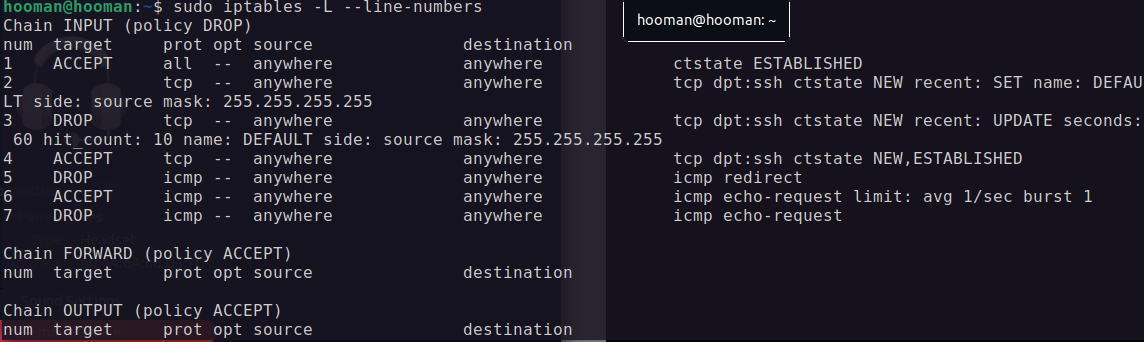
\includegraphics[scale=0.30]{pics/iptables5.png}
\end{center}